\documentclass[11pt,titlepage]{article}

\usepackage{geometry}
\usepackage{float}
\usepackage{graphicx}
\geometry{a4paper}
\geometry{margin=2cm}
\geometry{portrait}

\newcommand{\horrule}[1]{\rule{\linewidth}{#1}}

\title{
		\normalfont \normalsize \textsc{Client Name: DVT} \\
		\normalfont \normalsize \textsc{Project Name: KinderFinder} \\ [25pt]
		\horrule{0.5pt} \\[0.4cm]
		\huge Architecture Requirements \\
		\horrule{2pt} \\[0.5cm]
}
\author{\begin{tabular}{rl}
	\texttt{Team Name:} & \texttt{MAU Technologies} \\[0.5cm]
	Uteshlen Nadesan & 28163304 \\
	Michael Johnston & 12053300 \\
	Po-Han Chiu & 11063612
\end{tabular}
	\\ \\ \texttt{https://github.com/MrBean355/KinderFinder.git}
	\\ \\ \texttt{Version: 1}
%	\\ \\ \texttt{Change History:}
%	\\ The Summary here.
	}
\date{03 October 2014} 

\begin{document}
\maketitle
\tableofcontents
\newpage

\section{Access Channel Requirements}
The system's services are to be accessed through the following channels:
\begin{itemize}
\item \textbf{Web Portal}. Accessed through a web browser. This is where the system administration is done, as well as report viewing.
\item \textbf{Mobile App}. Accessed on Android devices. The parents who are monitoring their children will view their location on the app.
\end{itemize}

\section{Quality Requirements}
There are numerous quality requirements that are quantifiable:
\begin{itemize}
\item \textbf{Performance.} The system needs to give real-time information of where the child is now, not a minute ago. As soon as the child leaves the area, the parents need to be notified.
\item \textbf{Reliability.} It is critical that parents using the system can rely on it, because they want to be certain where their children are at all times. The system must always report the correct location of the transmitters.
\item \textbf{Scalability.} It needs to be easy to add or remove hardware to/from the system, so that restaurants can expand or shrink their monitoring zones with little effort and cost.
\item \textbf{Flexibility.} Different restaurants should be able to have their system customised to their needs, so they can use the system to its full potential.
\item \textbf{Maintainability.} The hardware and software components need to be easily accessible so that maintenance can be performed efficiently. The web administration portal must allow the users to easily maintain the system.
\item \textbf{Auditability.} The system will have a reporting module that must report statistics such as which zones are most popular and whether any devices are damaged.
\item \textbf{Integrability.} The system must be easily integrable with different hardware, not locked to one model.
\item \textbf{Cost.} The major cost of the system will be attributed to the hardware, such as RFID wristbands and receivers. The hardware must be affordable but decent quality, so that it can be relied upon without costing fortunes.
\item \textbf{Usability.} This could be measured by means of a survey, to find out how user-friendly the users find the system.
\end{itemize}

\section{Integration Requirements}
The system does not need to integrate with any external systems. However, since we are focusing on the software side, the hardware can be integrated with the software in the future (possibly by us if we have the time). For this, the hardware (RFID transmitters and receivers) must be integrated into the system, replacing any dummy "hardware" in place.

\section{Architecture Constraints}
The technologies that must be used are as follows:
\begin{itemize}
\item Microsoft SQL Server 2012 Express
\item Xamarin (Android app)
\item Microsoft Visual Studio 2013
\item ASP.NET MVC 5 \& WebAPI
\item C\#, HTML 5, JavaScript
\item Entity Framework (ORM)
\end{itemize}
The architecture as provided by the client is as follows:
\begin{figure}[H]
\begin{center}
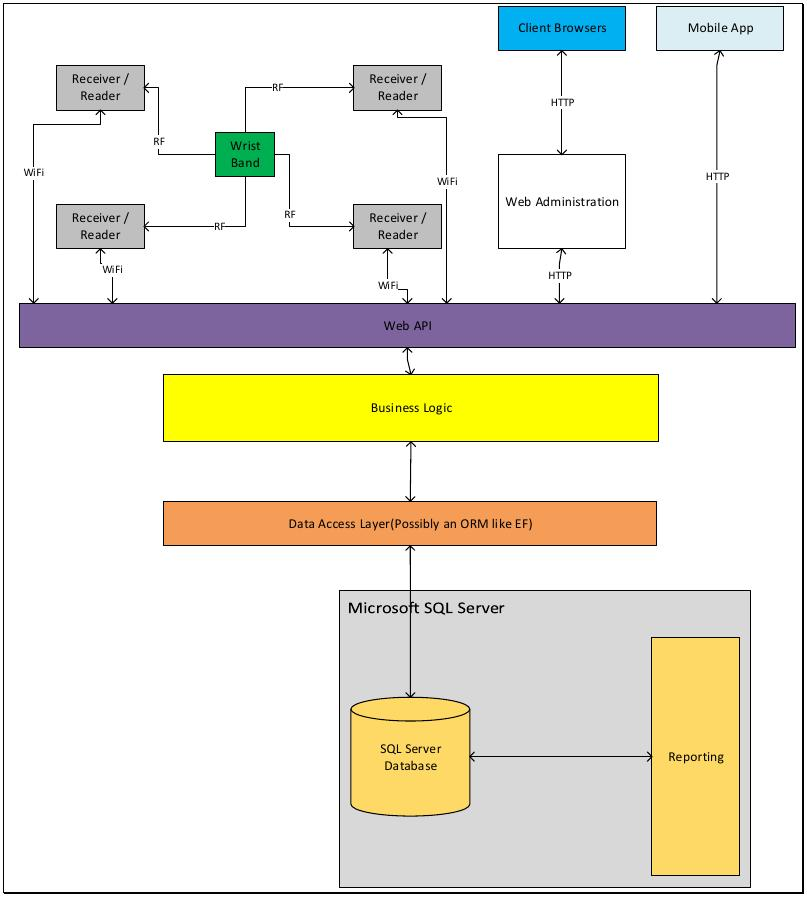
\includegraphics[scale=0.8]{SystemArchitecture.jpg}
\caption{System architecture.}
\end{center}
\end{figure}
\end{document}
